% documentclass: article used for scientific journals, short reports, program documentation, etc
% options: fontsize 11, generate document for double sided printing, a4-paper
\documentclass[aspectratio=169]{beamer}

% package for changing page layout
% \usepackage{geometry}
% \geometry{a4paper, lmargin=40mm, rmargin=45mm, tmargin=40mm, bmargin=45mm}
% set indentation
% \setlength{\parindent}{1em}
% set factor for line spacing
% \linespread{1.0}\selectfont
% set (dynamic) additional line spacing
% \setlength{\parskip}{1ex plus 0.5ex minus 0.3ex}

% rigorous formatting (not too much hyphens)
% \fussy
% \sloppy

% package for changing page layout (used to indent whole paragraphs with adjustwidth)
\usepackage{changepage}

% input encoding for special characters (e.g. ä,ü,ö,ß), only for non english text
% options: utf8 as encoding standard, latin1
\usepackage[utf8]{inputenc}
% package for font encoding
\usepackage[T1]{fontenc}
% package for changing used language (especially for more than one language)
% options: ngerman (new spelling) or default: english
\usepackage[ngerman]{babel}
% package for times font
% \usepackage{times}
% package for latin modern fonts
\usepackage{lmodern}

% package for math symbols, functions and environments from ams(american mathematical society)
\usepackage{amsmath}
\usepackage{mathtools}
% package for extended symbols from ams
\usepackage{amssymb}
% package for math black board symbols (e.g. R,Q,Z,...)
\usepackage{bbm}
\usepackage{mathrsfs}
% package for extended symbols from stmaryrd(st mary road)
\usepackage{stmaryrd}

% pack­age im­ple­ments scal­ing of the math ex­ten­sion font cmex; used for scaling math signs
\usepackage{exscale}

% package for including extern graphics plus scaling and rotating
\usepackage{graphicx}
%package for positioning figures
\usepackage{float}
% package for changing color of font and paper
% options: using names of default colors (e.g red, black)
% \usepackage[usenames]{color}
% \usepackage[dvipsnames]{xcolor}
\definecolor{shadecolor}{gray}{0.9}
\definecolor{MidnightBlue}{rgb}{0.3, 0.3, 0.9}
\definecolor{Red}{rgb}{1, 0, 0}
\definecolor{Black}{rgb}{0, 0, 0}
% package for customising captions
\usepackage[footnotesize, hang]{caption}
% package for customising enumerations (e.g. axioms)
\usepackage{enumitem}
% calc package reimplements \setcounter, \addtocounter, \setlength and \addtolength: commands now accept an infix notation expression
\usepackage{calc}
% package for creating framed, shaded, or differently highlighted regions that can break across pages; environments: framed, oframed, shaded, shaded*, snugshade, snugshade*, leftbar, titled-frame
\usepackage{framed}
% package for creating custom "list of"
% options: titles: do not intefere with standard headings for "list of"
% \usepackage[titles]{tocloft}


% change enumeration style of equations
% \renewcommand\theequation{\thesection.\arabic{equation}}

% init list of math for definitions and theorems
% \newcommand{\listofmathcall}{Verzeichnis der Definitionen und Sätze}
% \newlistof{math}{mathlist}{\listofmathcall}
% add parentheses around argument
\newcommand{\parent}[1]{ \ifx&#1&\else (#1) \fi }
% unnumerated mathematical definition environment definiton
\newenvironment{mathdef*}[2]{
	\begin{framed}
	\noindent
	{ \fontfamily{ppl}\selectfont \textbf{\textsc{#1:}} } ~ #2 
	\par \hfill\\ 
	\fontfamily{lmr}\selectfont \itshape
}{
	\end{framed}
}
% definitions for numerated mathematical definition environment
\newcounter{mathdefc}[section]
\newcommand*{\mathdefnum}{\thesection.\arabic{mathdefc}}
\renewcommand{\themathdefc}{\mathdefnum}
\newenvironment{mathdef}[2]{
	\refstepcounter{mathdefc}
	\addcontentsline{mathlist}{figure}{\protect{\numberline{\mathdefnum}#1 ~ #2}}
	\begin{mathdef*}{#1 \mathdefnum}{#2}
}{
	\end{mathdef*}
}
% standard mathdef calls
\newcommand{\definitioncall}{Definition}
\newenvironment{stddef*}[1][]{ \begin{mathdef*}{\definitioncall}{\parent{#1}} }{ \end{mathdef*} }
\newenvironment{stddef}[1][]{ \begin{mathdef}{\definitioncall}{\parent{#1}} }{ \end{mathdef} }
% unnumerated theorem environment definition
\newenvironment{maththeorem*}[2]{
	\begin{leftbar}
	\noindent
	{ \fontfamily{ppl}\selectfont \textbf{\textsc{#1:}} } ~ #2
	\par \hfill\\ 
	\fontfamily{lmr} \fontshape{it} \selectfont
}{ 
	\end{leftbar}
}
% definitions for numerated theorem environment
\newcounter{maththeoremc}[section]
\newcommand*\maththeoremnum{\thesection.\arabic{maththeoremc}}
\renewcommand{\themaththeoremc}{\maththeoremnum}
\newenvironment{maththeorem}[2]{
	\refstepcounter{maththeoremc}
	\addcontentsline{mathlist}{figure}{\protect{\qquad\numberline{\maththeoremnum}#1 ~ #2}}
	\begin{maththeorem*}{#1 \maththeoremnum}{#2}
}{
	\end{maththeorem*}
}
% standard maththeorem calls
\newcommand{\theoremcall}{Theorem}
\newenvironment{theorem*}[1][]{ \begin{maththeorem*}{\theoremcall}{\parent{#1}} }{ \end{maththeorem*} }
\renewenvironment{theorem}[1][]{ \begin{maththeorem}{\theoremcall}{\parent{#1}} }{ \end{maththeorem} }
\newcommand{\lemmacall}{Lemma}
\newenvironment{lemma*}[1][]{ \begin{maththeorem*}{\lemmacall}{\parent{#1}} }{ \end{maththeorem*} }
\renewenvironment{lemma}[1][]{ \begin{maththeorem}{\lemmacall}{\parent{#1}} }{ \end{maththeorem} }
\newcommand{\propositioncall}{Proposition}
\newenvironment{proposition*}[1][]{ \begin{maththeorem*}{\propositioncall}{\parent{#1}} }{ \end{maththeorem*} }
\newenvironment{proposition}[1][]{ \begin{maththeorem}{\propositioncall}{\parent{#1}} }{ \end{maththeorem} }
\newcommand{\corollarycall}{Korollar}
\newenvironment{corollary*}[1][]{ \begin{maththeorem*}{\corollarycall}{\parent{#1}} }{ \end{maththeorem*} }
\renewenvironment{corollary}[1][]{ \begin{maththeorem}{\corollarycall}{\parent{#1}} }{ \end{maththeorem} }
% q.e.d. definition
\renewcommand{\qed}{ \par \hfill \fontfamily{lmr} \fontshape{it} \selectfont \mbox{q.e.d.} \\}
\newcommand{\qedbox}{ \par \hfill $\Box$ \\ }
% proof environment definition for theorems
\newenvironment{mathproof}[1]{
	\par\hfill\\
	\noindent
	{ \fontfamily{lmr}\selectfont \small \textsc{#1:}}
	\normalfont
	\small
	\begin{adjustwidth}{1em}{}
	\medskip
}{ 
	\end{adjustwidth} 
	\qedbox
}
% standard mathproof calls
\newcommand{\proofcall}{Beweis}
\renewenvironment{proof}{ \begin{mathproof}{\proofcall} }{ \end{mathproof} }
\newcommand{\proofideacall}{Beweisidee}
\newenvironment{proofidea}{ \begin{mathproof}{\proofideacall} }{ \end{mathproof} }

% new displaymath command, so that equations will not be stretched
\newcommand{\D}[1]{\mbox{$ #1 $}}
% make unnumerated equation
\newcommand{\E}[1]{\[ #1 \]}
% command for curly brackets
\newcommand{\curlb}[1]{\left\{ #1 \right\}}
% command for box brackets
\newcommand{\boxb}[1]{\left[ #1 \right]}
% command for parentheses/curved brackets
\newcommand{\curvb}[1]{\left( #1 \right)}
% command for angle brackets
\newcommand{\angleb}[1]{\left\langle #1 \right\rangle}
% command for floor brackets
\newcommand{\floorb}[1]{\left\lfloor #1 \right\rfloor}
% command for ceil brackets
\newcommand{\ceilb}[1]{\left\lceil #1 \right\rceil}
% command for creating sets
\newcommand{\set}[2]{ \left\{ #1 \enspace \middle\vert \enspace #2 \right\} }
% command for absolute value
\newcommand{\abs}[1]{\left\vert #1 \right\vert}
\newcommand{\norm}[1]{\left\| #1 \right\|}
% commands for writing limits
\newcommand{\limit}[3]{\, \longrightarrow \, #1, \ #2 \longrightarrow #3}
\newcommand{\Limit}[2]{\lim_{#1 \rightarrow #2}}
% command for differential
\newcommand{\diff}{\mathrm{d}}
\newcommand{\Diff}{\mathrm{D}}
% command for derivative
% \newcommand{\Deriv}[3][]{\Diff_{#2}^{#1}#3}
% \newcommand{\deriv}[3][]{\dfrac{\diff^{#1}#2(#3)}{\diff #3^{#1}}}
\DeclareMathOperator{\Deriv}{\m{D}}

% command for integral
\newcommand{\integral}[4]{\int_{#1}^{#2} #3\ \diff #4}
\newcommand{\Integral}[4]{\int\limits_{#1}^{#2} #3\ \diff #4}
\newcommand{\iintegral}[2]{\int #1\ \diff #2} % indefinite integral
% mathematical definitions (standard sets)
\newcommand{\SR}{\mathds{R}} % real numbers
\newcommand{\SC}{\mathds{C}} % complex numbers
\newcommand{\SN}{\mathds{N}} % natural numbers
\newcommand{\SZ}{\mathds{Z}} % integral numbers
\newcommand{\SQ}{\mathds{Q}} % rational numbers
\newcommand{\SP}{\mathcal{P}} % power set
\newcommand{\SFP}{\mathds{P}} % polynom functions
\newcommand{\SFC}{\mathrm{C}} % complex valued functions (continous or differentiable)
\newcommand{\SFL}{\mathcal{L}} % space of integrable functions
\newcommand{\SFLL}{\mathrm{L}} % space of integrable function classes
\newcommand{\SH}{\mathcal{H}} % hilbert space
% mathematical standard functions
\DeclareMathOperator{\real}{Re} % real part
\DeclareMathOperator{\imag}{Im} % imaginary part
\newcommand{\FF}{\mathcal{F}} % fourier transform
\newcommand{\FE}{\mathbb{E}} % expectation
\DeclareMathOperator{\var}{var} % variance
\newcommand{\FN}{\mathcal{N}} % normal distribution

% command for physical units
\newcommand{\unit}[1]{\, \mathrm{#1}}

% \usepackage{calrsfs}
% \DeclareMathAlphabet{\pazocal}{OMS}{zplm}{m}{n}
\usepackage{mathrsfs}

% package for init listings(non-formatted  text) e.g. different source codes
\usepackage{listings}


% definitions for listing colors
\definecolor{codeDarkGray}{gray}{0.2}
\definecolor{codeGray}{gray}{0.4}
\definecolor{codeLightGray}{gray}{0.9}
% predefinitions for listings
\newcommand{\listingcall}{Listing}
\newlength{\listingframemargin}
\setlength{\listingframemargin}{1em}
\newlength{\listingmargin}
\setlength{\listingmargin}{0.1\textwidth}
% \newlength{\listingwidth}
% \setlength{\listingwidth}{ ( \textwidth - \listingmargin * \real{2} + \listingframemargin * \real{2} ) }
% definitions for list of listings
\newcommand{\listoflistingscall}{\listingcall -Verzeichnis}
% \newlistof{listings}{listinglist}{\listoflistingscall}
% style definition for standard code listings
\lstdefinestyle{std}{
	belowcaptionskip=0.5\baselineskip,
	breaklines=true,
	frameround=tttt,
	frame=tblr,
	xleftmargin=0em,
	xrightmargin=0em,
	showstringspaces=false,
	showtabs=false,
	% tab=\smash{\rule[-.2\baselineskip]{.4pt}{\baselineskip}\kern.5em},
	basicstyle= \fontfamily{pcr}\selectfont\footnotesize\bfseries,
	keywordstyle= \bfseries\color{MidnightBlue}, %\color{codeDarkGray},
	commentstyle= \itshape\color{codeGray},
	identifierstyle=\color{codeDarkGray},
	stringstyle=\color{BurntOrange}, %\color{codeDarkGray},
	numberstyle=\tiny\ttfamily,
	% numbers=left,
	numbersep = 2em,
	% numberstep = 5,
	% captionpos=t,
	tabsize=4,
	backgroundcolor=\color{codeLightGray},
	framexleftmargin=\listingframemargin,
	framexrightmargin=\listingframemargin
}
% definition for unnumerated listing
\newcommand{\inputlistingn}[3][]{
	\begin{center}
		\begin{adjustwidth}{\listingmargin}{\listingmargin}
			\centerline{ {\fontfamily{lmr}\selectfont\scshape \listingcall:}\quad #2 }
			\lstinputlisting[style=std, #1]{#3}
		\end{adjustwidth}
	\end{center}
}
% definition for numerated listing
\newcounter{listingc}[section]
\newcommand*\listingnum{\thesection.\arabic{listingc}}
\renewcommand{\thelistingc}{\listingnum}
\newcommand{\inputlisting}[3][]{
	\refstepcounter{listingc}
	\addcontentsline{listinglist}{figure}{\protect{\numberline{\listingnum:} #2 } }
	\inputlistingn[#1]{#2}{#3}
}


% package for including csv-tables from file
% \usepackage{csvsimple}
% package for creating, loading and manipulating databases
\usepackage{datatool}

% package for converting eps-files to pdf-files and then include them
\usepackage{epstopdf}
% use another program (ps2pdf) for converting
% !!! important: set shell_escape=1 in /etc/texmf/texmf.cnf (Linux/Ubuntu 12.04) for allowing to use other programs
% !!!			or use the command line with -shell-escape
% \epstopdfDeclareGraphicsRule{.eps}{pdf}{.pdf}{
% ps2pdf -dEPSCrop #1 \OutputFile
% }


% package for reference to last page (output number of last page)
\usepackage{lastpage}
% package for using header and footer
% options: automate terms of right and left marks
\usepackage[automark]{scrpage2}
% \setlength{\headheight}{4\baselineskip}
% set style for footer and header
% \pagestyle{scrheadings}
% \pagestyle{headings}
% clear pagestyle for redefining
% \clearscrheadfoot
% set header and footer: use <xx>head/foot[]{Text} (i...inner, o...outer, c...center, o...odd, e...even, l...left, r...right)
% \ihead[]{Fast Fourier Transform}
% \ohead[]{Markus Pawellek \\ markuspawellek@gmail.com}
% \cfoot[]{\newline\newline\newline\pagemark}
% use that for mark to last page: \pageref{LastPage}
% set header separation line
% \setheadsepline[\textwidth]{0.5pt}
% set foot separation line
% \setfootsepline[\textwidth]{0.5pt}

\usepackage{tcolorbox}
% \usepackage{tikz}
% \tcbuselibrary{listings}
\tcbuselibrary{many}

\usefonttheme[onlymath]{serif}

% package for more math blackboard symbols
\usepackage{dsfont}

% pack­age im­ple­ments scal­ing of the math ex­ten­sion font cmex; used for scaling math signs
\usepackage{exscale}

\usepackage{enumitem}
\usepackage{array}
% \usepackage{natbib}
% \bibliographystyle{plain}
\usepackage{url}

\newcommand{\m}[1]{\mathrm{#1}}
\newcommand{\transp}[1]{{#1}^\m{T}}
\newcommand{\idmat}{\m{I}}


\title{Seminar Numerische Verfahren: \\ Nichtlineare Ausgleichsprobleme}
\author{Kazimir Menzel \\ Markus Pawellek}
% \date{03.Februar 2016}

\begin{document}
	
	\frame{\maketitle}


	\begin{frame}
		\begin{tcolorbox}
			\begin{figure}
				% GNUPLOT: LaTeX picture with Postscript
\begingroup
  \makeatletter
  \providecommand\color[2][]{%
    \GenericError{(gnuplot) \space\space\space\@spaces}{%
      Package color not loaded in conjunction with
      terminal option `colourtext'%
    }{See the gnuplot documentation for explanation.%
    }{Either use 'blacktext' in gnuplot or load the package
      color.sty in LaTeX.}%
    \renewcommand\color[2][]{}%
  }%
  \providecommand\includegraphics[2][]{%
    \GenericError{(gnuplot) \space\space\space\@spaces}{%
      Package graphicx or graphics not loaded%
    }{See the gnuplot documentation for explanation.%
    }{The gnuplot epslatex terminal needs graphicx.sty or graphics.sty.}%
    \renewcommand\includegraphics[2][]{}%
  }%
  \providecommand\rotatebox[2]{#2}%
  \@ifundefined{ifGPcolor}{%
    \newif\ifGPcolor
    \GPcolorfalse
  }{}%
  \@ifundefined{ifGPblacktext}{%
    \newif\ifGPblacktext
    \GPblacktexttrue
  }{}%
  % define a \g@addto@macro without @ in the name:
  \let\gplgaddtomacro\g@addto@macro
  % define empty templates for all commands taking text:
  \gdef\gplbacktext{}%
  \gdef\gplfronttext{}%
  \makeatother
  \ifGPblacktext
    % no textcolor at all
    \def\colorrgb#1{}%
    \def\colorgray#1{}%
  \else
    % gray or color?
    \ifGPcolor
      \def\colorrgb#1{\color[rgb]{#1}}%
      \def\colorgray#1{\color[gray]{#1}}%
      \expandafter\def\csname LTw\endcsname{\color{white}}%
      \expandafter\def\csname LTb\endcsname{\color{black}}%
      \expandafter\def\csname LTa\endcsname{\color{black}}%
      \expandafter\def\csname LT0\endcsname{\color[rgb]{1,0,0}}%
      \expandafter\def\csname LT1\endcsname{\color[rgb]{0,1,0}}%
      \expandafter\def\csname LT2\endcsname{\color[rgb]{0,0,1}}%
      \expandafter\def\csname LT3\endcsname{\color[rgb]{1,0,1}}%
      \expandafter\def\csname LT4\endcsname{\color[rgb]{0,1,1}}%
      \expandafter\def\csname LT5\endcsname{\color[rgb]{1,1,0}}%
      \expandafter\def\csname LT6\endcsname{\color[rgb]{0,0,0}}%
      \expandafter\def\csname LT7\endcsname{\color[rgb]{1,0.3,0}}%
      \expandafter\def\csname LT8\endcsname{\color[rgb]{0.5,0.5,0.5}}%
    \else
      % gray
      \def\colorrgb#1{\color{black}}%
      \def\colorgray#1{\color[gray]{#1}}%
      \expandafter\def\csname LTw\endcsname{\color{white}}%
      \expandafter\def\csname LTb\endcsname{\color{black}}%
      \expandafter\def\csname LTa\endcsname{\color{black}}%
      \expandafter\def\csname LT0\endcsname{\color{black}}%
      \expandafter\def\csname LT1\endcsname{\color{black}}%
      \expandafter\def\csname LT2\endcsname{\color{black}}%
      \expandafter\def\csname LT3\endcsname{\color{black}}%
      \expandafter\def\csname LT4\endcsname{\color{black}}%
      \expandafter\def\csname LT5\endcsname{\color{black}}%
      \expandafter\def\csname LT6\endcsname{\color{black}}%
      \expandafter\def\csname LT7\endcsname{\color{black}}%
      \expandafter\def\csname LT8\endcsname{\color{black}}%
    \fi
  \fi
  \setlength{\unitlength}{0.0500bp}%
  \begin{picture}(6802.00,3968.00)%
    \gplgaddtomacro\gplbacktext{%
      \csname LTb\endcsname%
      \put(814,704){\makebox(0,0)[r]{\strut{} 0}}%
      \put(814,1037){\makebox(0,0)[r]{\strut{} 2}}%
      \put(814,1370){\makebox(0,0)[r]{\strut{} 4}}%
      \put(814,1704){\makebox(0,0)[r]{\strut{} 6}}%
      \put(814,2037){\makebox(0,0)[r]{\strut{} 8}}%
      \put(814,2370){\makebox(0,0)[r]{\strut{} 10}}%
      \put(814,2703){\makebox(0,0)[r]{\strut{} 12}}%
      \put(814,3037){\makebox(0,0)[r]{\strut{} 14}}%
      \put(814,3370){\makebox(0,0)[r]{\strut{} 16}}%
      \put(814,3703){\makebox(0,0)[r]{\strut{} 18}}%
      \put(946,484){\makebox(0,0){\strut{} 0}}%
      \put(1492,484){\makebox(0,0){\strut{} 1}}%
      \put(2038,484){\makebox(0,0){\strut{} 2}}%
      \put(2584,484){\makebox(0,0){\strut{} 3}}%
      \put(3130,484){\makebox(0,0){\strut{} 4}}%
      \put(3676,484){\makebox(0,0){\strut{} 5}}%
      \put(4221,484){\makebox(0,0){\strut{} 6}}%
      \put(4767,484){\makebox(0,0){\strut{} 7}}%
      \put(5313,484){\makebox(0,0){\strut{} 8}}%
      \put(5859,484){\makebox(0,0){\strut{} 9}}%
      \put(6405,484){\makebox(0,0){\strut{} 10}}%
      \put(176,2203){\rotatebox{-270}{\makebox(0,0){\strut{}$y$}}}%
      \put(3675,154){\makebox(0,0){\strut{}$x$}}%
    }%
    \gplgaddtomacro\gplfronttext{%
      \csname LTb\endcsname%
      \put(1870,3398){\makebox(0,0)[r]{\strut{}\footnotesize Messwerte}}%
    }%
    \gplbacktext
    \put(0,0){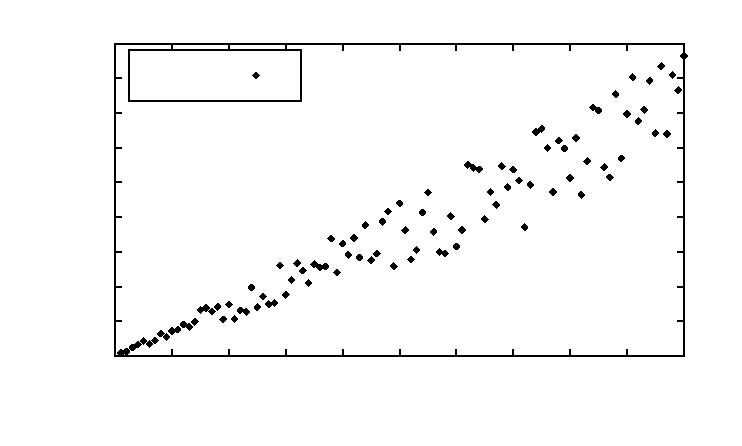
\includegraphics{lin-fit-example-data}}%
    \gplfronttext
  \end{picture}%
\endgroup

			\end{figure}
		\end{tcolorbox}
	\end{frame}
	
	\begin{frame}
		\begin{tcolorbox}
			\begin{figure}
				% GNUPLOT: LaTeX picture with Postscript
\begingroup
  \makeatletter
  \providecommand\color[2][]{%
    \GenericError{(gnuplot) \space\space\space\@spaces}{%
      Package color not loaded in conjunction with
      terminal option `colourtext'%
    }{See the gnuplot documentation for explanation.%
    }{Either use 'blacktext' in gnuplot or load the package
      color.sty in LaTeX.}%
    \renewcommand\color[2][]{}%
  }%
  \providecommand\includegraphics[2][]{%
    \GenericError{(gnuplot) \space\space\space\@spaces}{%
      Package graphicx or graphics not loaded%
    }{See the gnuplot documentation for explanation.%
    }{The gnuplot epslatex terminal needs graphicx.sty or graphics.sty.}%
    \renewcommand\includegraphics[2][]{}%
  }%
  \providecommand\rotatebox[2]{#2}%
  \@ifundefined{ifGPcolor}{%
    \newif\ifGPcolor
    \GPcolorfalse
  }{}%
  \@ifundefined{ifGPblacktext}{%
    \newif\ifGPblacktext
    \GPblacktexttrue
  }{}%
  % define a \g@addto@macro without @ in the name:
  \let\gplgaddtomacro\g@addto@macro
  % define empty templates for all commands taking text:
  \gdef\gplbacktext{}%
  \gdef\gplfronttext{}%
  \makeatother
  \ifGPblacktext
    % no textcolor at all
    \def\colorrgb#1{}%
    \def\colorgray#1{}%
  \else
    % gray or color?
    \ifGPcolor
      \def\colorrgb#1{\color[rgb]{#1}}%
      \def\colorgray#1{\color[gray]{#1}}%
      \expandafter\def\csname LTw\endcsname{\color{white}}%
      \expandafter\def\csname LTb\endcsname{\color{black}}%
      \expandafter\def\csname LTa\endcsname{\color{black}}%
      \expandafter\def\csname LT0\endcsname{\color[rgb]{1,0,0}}%
      \expandafter\def\csname LT1\endcsname{\color[rgb]{0,1,0}}%
      \expandafter\def\csname LT2\endcsname{\color[rgb]{0,0,1}}%
      \expandafter\def\csname LT3\endcsname{\color[rgb]{1,0,1}}%
      \expandafter\def\csname LT4\endcsname{\color[rgb]{0,1,1}}%
      \expandafter\def\csname LT5\endcsname{\color[rgb]{1,1,0}}%
      \expandafter\def\csname LT6\endcsname{\color[rgb]{0,0,0}}%
      \expandafter\def\csname LT7\endcsname{\color[rgb]{1,0.3,0}}%
      \expandafter\def\csname LT8\endcsname{\color[rgb]{0.5,0.5,0.5}}%
    \else
      % gray
      \def\colorrgb#1{\color{black}}%
      \def\colorgray#1{\color[gray]{#1}}%
      \expandafter\def\csname LTw\endcsname{\color{white}}%
      \expandafter\def\csname LTb\endcsname{\color{black}}%
      \expandafter\def\csname LTa\endcsname{\color{black}}%
      \expandafter\def\csname LT0\endcsname{\color{black}}%
      \expandafter\def\csname LT1\endcsname{\color{black}}%
      \expandafter\def\csname LT2\endcsname{\color{black}}%
      \expandafter\def\csname LT3\endcsname{\color{black}}%
      \expandafter\def\csname LT4\endcsname{\color{black}}%
      \expandafter\def\csname LT5\endcsname{\color{black}}%
      \expandafter\def\csname LT6\endcsname{\color{black}}%
      \expandafter\def\csname LT7\endcsname{\color{black}}%
      \expandafter\def\csname LT8\endcsname{\color{black}}%
    \fi
  \fi
  \setlength{\unitlength}{0.0500bp}%
  \begin{picture}(6802.00,3968.00)%
    \gplgaddtomacro\gplbacktext{%
      \csname LTb\endcsname%
      \put(814,704){\makebox(0,0)[r]{\strut{} 0}}%
      \put(814,1037){\makebox(0,0)[r]{\strut{} 2}}%
      \put(814,1370){\makebox(0,0)[r]{\strut{} 4}}%
      \put(814,1704){\makebox(0,0)[r]{\strut{} 6}}%
      \put(814,2037){\makebox(0,0)[r]{\strut{} 8}}%
      \put(814,2370){\makebox(0,0)[r]{\strut{} 10}}%
      \put(814,2703){\makebox(0,0)[r]{\strut{} 12}}%
      \put(814,3037){\makebox(0,0)[r]{\strut{} 14}}%
      \put(814,3370){\makebox(0,0)[r]{\strut{} 16}}%
      \put(814,3703){\makebox(0,0)[r]{\strut{} 18}}%
      \put(946,484){\makebox(0,0){\strut{} 0}}%
      \put(1492,484){\makebox(0,0){\strut{} 1}}%
      \put(2038,484){\makebox(0,0){\strut{} 2}}%
      \put(2584,484){\makebox(0,0){\strut{} 3}}%
      \put(3130,484){\makebox(0,0){\strut{} 4}}%
      \put(3676,484){\makebox(0,0){\strut{} 5}}%
      \put(4221,484){\makebox(0,0){\strut{} 6}}%
      \put(4767,484){\makebox(0,0){\strut{} 7}}%
      \put(5313,484){\makebox(0,0){\strut{} 8}}%
      \put(5859,484){\makebox(0,0){\strut{} 9}}%
      \put(6405,484){\makebox(0,0){\strut{} 10}}%
      \put(176,2203){\rotatebox{-270}{\makebox(0,0){\strut{}$y$}}}%
      \put(3675,154){\makebox(0,0){\strut{}$x$}}%
    }%
    \gplgaddtomacro\gplfronttext{%
      \csname LTb\endcsname%
      \put(2794,3398){\makebox(0,0)[r]{\strut{}\footnotesize Messwerte}}%
      \csname LTb\endcsname%
      \put(2794,3134){\makebox(0,0)[r]{\strut{}\footnotesize Ausgleichsgerade}}%
    }%
    \gplbacktext
    \put(0,0){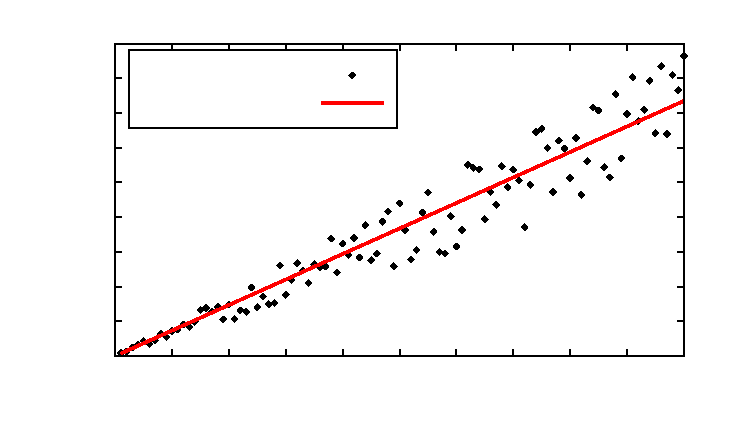
\includegraphics{lin-fit-example}}%
    \gplfronttext
  \end{picture}%
\endgroup

			\end{figure}
		\end{tcolorbox}
	\end{frame}

	\begin{frame}
		\begin{tcolorbox}
			\begin{figure}
				% GNUPLOT: LaTeX picture with Postscript
\begingroup
  \makeatletter
  \providecommand\color[2][]{%
    \GenericError{(gnuplot) \space\space\space\@spaces}{%
      Package color not loaded in conjunction with
      terminal option `colourtext'%
    }{See the gnuplot documentation for explanation.%
    }{Either use 'blacktext' in gnuplot or load the package
      color.sty in LaTeX.}%
    \renewcommand\color[2][]{}%
  }%
  \providecommand\includegraphics[2][]{%
    \GenericError{(gnuplot) \space\space\space\@spaces}{%
      Package graphicx or graphics not loaded%
    }{See the gnuplot documentation for explanation.%
    }{The gnuplot epslatex terminal needs graphicx.sty or graphics.sty.}%
    \renewcommand\includegraphics[2][]{}%
  }%
  \providecommand\rotatebox[2]{#2}%
  \@ifundefined{ifGPcolor}{%
    \newif\ifGPcolor
    \GPcolorfalse
  }{}%
  \@ifundefined{ifGPblacktext}{%
    \newif\ifGPblacktext
    \GPblacktexttrue
  }{}%
  % define a \g@addto@macro without @ in the name:
  \let\gplgaddtomacro\g@addto@macro
  % define empty templates for all commands taking text:
  \gdef\gplbacktext{}%
  \gdef\gplfronttext{}%
  \makeatother
  \ifGPblacktext
    % no textcolor at all
    \def\colorrgb#1{}%
    \def\colorgray#1{}%
  \else
    % gray or color?
    \ifGPcolor
      \def\colorrgb#1{\color[rgb]{#1}}%
      \def\colorgray#1{\color[gray]{#1}}%
      \expandafter\def\csname LTw\endcsname{\color{white}}%
      \expandafter\def\csname LTb\endcsname{\color{black}}%
      \expandafter\def\csname LTa\endcsname{\color{black}}%
      \expandafter\def\csname LT0\endcsname{\color[rgb]{1,0,0}}%
      \expandafter\def\csname LT1\endcsname{\color[rgb]{0,1,0}}%
      \expandafter\def\csname LT2\endcsname{\color[rgb]{0,0,1}}%
      \expandafter\def\csname LT3\endcsname{\color[rgb]{1,0,1}}%
      \expandafter\def\csname LT4\endcsname{\color[rgb]{0,1,1}}%
      \expandafter\def\csname LT5\endcsname{\color[rgb]{1,1,0}}%
      \expandafter\def\csname LT6\endcsname{\color[rgb]{0,0,0}}%
      \expandafter\def\csname LT7\endcsname{\color[rgb]{1,0.3,0}}%
      \expandafter\def\csname LT8\endcsname{\color[rgb]{0.5,0.5,0.5}}%
    \else
      % gray
      \def\colorrgb#1{\color{black}}%
      \def\colorgray#1{\color[gray]{#1}}%
      \expandafter\def\csname LTw\endcsname{\color{white}}%
      \expandafter\def\csname LTb\endcsname{\color{black}}%
      \expandafter\def\csname LTa\endcsname{\color{black}}%
      \expandafter\def\csname LT0\endcsname{\color{black}}%
      \expandafter\def\csname LT1\endcsname{\color{black}}%
      \expandafter\def\csname LT2\endcsname{\color{black}}%
      \expandafter\def\csname LT3\endcsname{\color{black}}%
      \expandafter\def\csname LT4\endcsname{\color{black}}%
      \expandafter\def\csname LT5\endcsname{\color{black}}%
      \expandafter\def\csname LT6\endcsname{\color{black}}%
      \expandafter\def\csname LT7\endcsname{\color{black}}%
      \expandafter\def\csname LT8\endcsname{\color{black}}%
    \fi
  \fi
  \setlength{\unitlength}{0.0500bp}%
  \begin{picture}(6802.00,3968.00)%
    \gplgaddtomacro\gplbacktext{%
      \csname LTb\endcsname%
      \put(946,954){\makebox(0,0)[r]{\strut{}-1}}%
      \put(946,1579){\makebox(0,0)[r]{\strut{}-0.5}}%
      \put(946,2204){\makebox(0,0)[r]{\strut{} 0}}%
      \put(946,2828){\makebox(0,0)[r]{\strut{} 0.5}}%
      \put(946,3453){\makebox(0,0)[r]{\strut{} 1}}%
      \put(1078,484){\makebox(0,0){\strut{} 0}}%
      \put(2123,484){\makebox(0,0){\strut{} 2}}%
      \put(3167,484){\makebox(0,0){\strut{} 4}}%
      \put(4212,484){\makebox(0,0){\strut{} 6}}%
      \put(5256,484){\makebox(0,0){\strut{} 8}}%
      \put(6301,484){\makebox(0,0){\strut{} 10}}%
      \put(176,2203){\rotatebox{-270}{\makebox(0,0){\strut{}$y$}}}%
      \put(3741,154){\makebox(0,0){\strut{}$x$}}%
    }%
    \gplgaddtomacro\gplfronttext{%
      \csname LTb\endcsname%
      \put(5418,3398){\makebox(0,0)[r]{\strut{}\footnotesize Messwerte}}%
    }%
    \gplbacktext
    \put(0,0){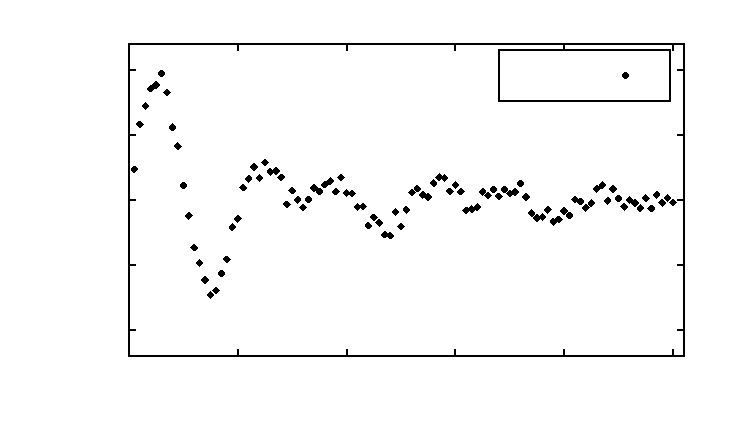
\includegraphics{nonlin-fit-example-data}}%
    \gplfronttext
  \end{picture}%
\endgroup

			\end{figure}
		\end{tcolorbox}
	\end{frame}
	
	\begin{frame}
	\begin{tcolorbox}
		\begin{figure}
				% GNUPLOT: LaTeX picture with Postscript
\begingroup
  \makeatletter
  \providecommand\color[2][]{%
    \GenericError{(gnuplot) \space\space\space\@spaces}{%
      Package color not loaded in conjunction with
      terminal option `colourtext'%
    }{See the gnuplot documentation for explanation.%
    }{Either use 'blacktext' in gnuplot or load the package
      color.sty in LaTeX.}%
    \renewcommand\color[2][]{}%
  }%
  \providecommand\includegraphics[2][]{%
    \GenericError{(gnuplot) \space\space\space\@spaces}{%
      Package graphicx or graphics not loaded%
    }{See the gnuplot documentation for explanation.%
    }{The gnuplot epslatex terminal needs graphicx.sty or graphics.sty.}%
    \renewcommand\includegraphics[2][]{}%
  }%
  \providecommand\rotatebox[2]{#2}%
  \@ifundefined{ifGPcolor}{%
    \newif\ifGPcolor
    \GPcolorfalse
  }{}%
  \@ifundefined{ifGPblacktext}{%
    \newif\ifGPblacktext
    \GPblacktexttrue
  }{}%
  % define a \g@addto@macro without @ in the name:
  \let\gplgaddtomacro\g@addto@macro
  % define empty templates for all commands taking text:
  \gdef\gplbacktext{}%
  \gdef\gplfronttext{}%
  \makeatother
  \ifGPblacktext
    % no textcolor at all
    \def\colorrgb#1{}%
    \def\colorgray#1{}%
  \else
    % gray or color?
    \ifGPcolor
      \def\colorrgb#1{\color[rgb]{#1}}%
      \def\colorgray#1{\color[gray]{#1}}%
      \expandafter\def\csname LTw\endcsname{\color{white}}%
      \expandafter\def\csname LTb\endcsname{\color{black}}%
      \expandafter\def\csname LTa\endcsname{\color{black}}%
      \expandafter\def\csname LT0\endcsname{\color[rgb]{1,0,0}}%
      \expandafter\def\csname LT1\endcsname{\color[rgb]{0,1,0}}%
      \expandafter\def\csname LT2\endcsname{\color[rgb]{0,0,1}}%
      \expandafter\def\csname LT3\endcsname{\color[rgb]{1,0,1}}%
      \expandafter\def\csname LT4\endcsname{\color[rgb]{0,1,1}}%
      \expandafter\def\csname LT5\endcsname{\color[rgb]{1,1,0}}%
      \expandafter\def\csname LT6\endcsname{\color[rgb]{0,0,0}}%
      \expandafter\def\csname LT7\endcsname{\color[rgb]{1,0.3,0}}%
      \expandafter\def\csname LT8\endcsname{\color[rgb]{0.5,0.5,0.5}}%
    \else
      % gray
      \def\colorrgb#1{\color{black}}%
      \def\colorgray#1{\color[gray]{#1}}%
      \expandafter\def\csname LTw\endcsname{\color{white}}%
      \expandafter\def\csname LTb\endcsname{\color{black}}%
      \expandafter\def\csname LTa\endcsname{\color{black}}%
      \expandafter\def\csname LT0\endcsname{\color{black}}%
      \expandafter\def\csname LT1\endcsname{\color{black}}%
      \expandafter\def\csname LT2\endcsname{\color{black}}%
      \expandafter\def\csname LT3\endcsname{\color{black}}%
      \expandafter\def\csname LT4\endcsname{\color{black}}%
      \expandafter\def\csname LT5\endcsname{\color{black}}%
      \expandafter\def\csname LT6\endcsname{\color{black}}%
      \expandafter\def\csname LT7\endcsname{\color{black}}%
      \expandafter\def\csname LT8\endcsname{\color{black}}%
    \fi
  \fi
  \setlength{\unitlength}{0.0500bp}%
  \begin{picture}(6802.00,3968.00)%
    \gplgaddtomacro\gplbacktext{%
      \csname LTb\endcsname%
      \put(946,954){\makebox(0,0)[r]{\strut{}-1}}%
      \put(946,1579){\makebox(0,0)[r]{\strut{}-0.5}}%
      \put(946,2204){\makebox(0,0)[r]{\strut{} 0}}%
      \put(946,2828){\makebox(0,0)[r]{\strut{} 0.5}}%
      \put(946,3453){\makebox(0,0)[r]{\strut{} 1}}%
      \put(1078,484){\makebox(0,0){\strut{} 0}}%
      \put(2123,484){\makebox(0,0){\strut{} 2}}%
      \put(3167,484){\makebox(0,0){\strut{} 4}}%
      \put(4212,484){\makebox(0,0){\strut{} 6}}%
      \put(5256,484){\makebox(0,0){\strut{} 8}}%
      \put(6301,484){\makebox(0,0){\strut{} 10}}%
      \put(176,2203){\rotatebox{-270}{\makebox(0,0){\strut{}$y$}}}%
      \put(3741,154){\makebox(0,0){\strut{}$x$}}%
    }%
    \gplgaddtomacro\gplfronttext{%
      \csname LTb\endcsname%
      \put(5418,3398){\makebox(0,0)[r]{\strut{}\footnotesize Messwerte}}%
      \csname LTb\endcsname%
      \put(5418,3134){\makebox(0,0)[r]{\strut{}\footnotesize $f(x) = \frac{\sin(ax)\sin(x)}{x}$}}%
    }%
    \gplbacktext
    \put(0,0){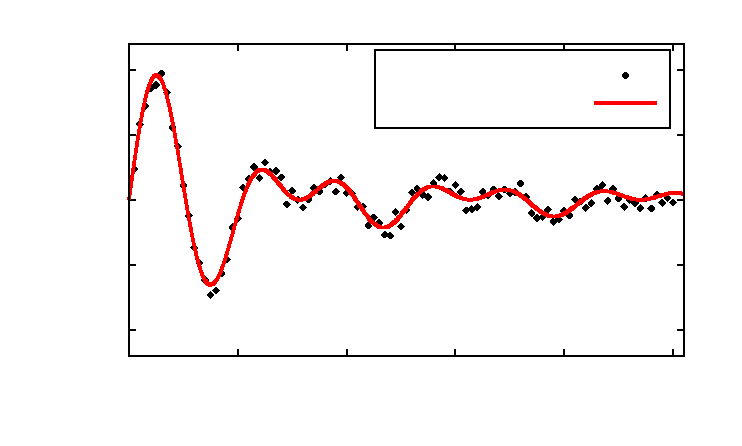
\includegraphics{nonlin-fit-example}}%
    \gplfronttext
  \end{picture}%
\endgroup

			\end{figure}
	\end{tcolorbox}
	\end{frame}


	\frame{\frametitle{Gliederung} \begin{adjustwidth}{1em}{}\tableofcontents\end{adjustwidth}}

	\section{Mathematische Grundlagen} % (fold)
	\label{sec:mathematische_grundlagen}
	
		\subsection{Idee des Ausgleichsproblems} % (fold)
		\label{sub:idee_des_ausgleichsproblems}

			\begin{frame}
				\frametitle{Idee des Ausgleichsproblems}

				\begin{tcolorbox}
					\begin{figure}
							% GNUPLOT: LaTeX picture with Postscript
\begingroup
  \makeatletter
  \providecommand\color[2][]{%
    \GenericError{(gnuplot) \space\space\space\@spaces}{%
      Package color not loaded in conjunction with
      terminal option `colourtext'%
    }{See the gnuplot documentation for explanation.%
    }{Either use 'blacktext' in gnuplot or load the package
      color.sty in LaTeX.}%
    \renewcommand\color[2][]{}%
  }%
  \providecommand\includegraphics[2][]{%
    \GenericError{(gnuplot) \space\space\space\@spaces}{%
      Package graphicx or graphics not loaded%
    }{See the gnuplot documentation for explanation.%
    }{The gnuplot epslatex terminal needs graphicx.sty or graphics.sty.}%
    \renewcommand\includegraphics[2][]{}%
  }%
  \providecommand\rotatebox[2]{#2}%
  \@ifundefined{ifGPcolor}{%
    \newif\ifGPcolor
    \GPcolorfalse
  }{}%
  \@ifundefined{ifGPblacktext}{%
    \newif\ifGPblacktext
    \GPblacktexttrue
  }{}%
  % define a \g@addto@macro without @ in the name:
  \let\gplgaddtomacro\g@addto@macro
  % define empty templates for all commands taking text:
  \gdef\gplbacktext{}%
  \gdef\gplfronttext{}%
  \makeatother
  \ifGPblacktext
    % no textcolor at all
    \def\colorrgb#1{}%
    \def\colorgray#1{}%
  \else
    % gray or color?
    \ifGPcolor
      \def\colorrgb#1{\color[rgb]{#1}}%
      \def\colorgray#1{\color[gray]{#1}}%
      \expandafter\def\csname LTw\endcsname{\color{white}}%
      \expandafter\def\csname LTb\endcsname{\color{black}}%
      \expandafter\def\csname LTa\endcsname{\color{black}}%
      \expandafter\def\csname LT0\endcsname{\color[rgb]{1,0,0}}%
      \expandafter\def\csname LT1\endcsname{\color[rgb]{0,1,0}}%
      \expandafter\def\csname LT2\endcsname{\color[rgb]{0,0,1}}%
      \expandafter\def\csname LT3\endcsname{\color[rgb]{1,0,1}}%
      \expandafter\def\csname LT4\endcsname{\color[rgb]{0,1,1}}%
      \expandafter\def\csname LT5\endcsname{\color[rgb]{1,1,0}}%
      \expandafter\def\csname LT6\endcsname{\color[rgb]{0,0,0}}%
      \expandafter\def\csname LT7\endcsname{\color[rgb]{1,0.3,0}}%
      \expandafter\def\csname LT8\endcsname{\color[rgb]{0.5,0.5,0.5}}%
    \else
      % gray
      \def\colorrgb#1{\color{black}}%
      \def\colorgray#1{\color[gray]{#1}}%
      \expandafter\def\csname LTw\endcsname{\color{white}}%
      \expandafter\def\csname LTb\endcsname{\color{black}}%
      \expandafter\def\csname LTa\endcsname{\color{black}}%
      \expandafter\def\csname LT0\endcsname{\color{black}}%
      \expandafter\def\csname LT1\endcsname{\color{black}}%
      \expandafter\def\csname LT2\endcsname{\color{black}}%
      \expandafter\def\csname LT3\endcsname{\color{black}}%
      \expandafter\def\csname LT4\endcsname{\color{black}}%
      \expandafter\def\csname LT5\endcsname{\color{black}}%
      \expandafter\def\csname LT6\endcsname{\color{black}}%
      \expandafter\def\csname LT7\endcsname{\color{black}}%
      \expandafter\def\csname LT8\endcsname{\color{black}}%
    \fi
  \fi
  \setlength{\unitlength}{0.0500bp}%
  \begin{picture}(6802.00,3968.00)%
    \gplgaddtomacro\gplbacktext{%
      \csname LTb\endcsname%
      \put(946,954){\makebox(0,0)[r]{\strut{}-1}}%
      \put(946,1579){\makebox(0,0)[r]{\strut{}-0.5}}%
      \put(946,2204){\makebox(0,0)[r]{\strut{} 0}}%
      \put(946,2828){\makebox(0,0)[r]{\strut{} 0.5}}%
      \put(946,3453){\makebox(0,0)[r]{\strut{} 1}}%
      \put(1078,484){\makebox(0,0){\strut{} 0}}%
      \put(2123,484){\makebox(0,0){\strut{} 2}}%
      \put(3167,484){\makebox(0,0){\strut{} 4}}%
      \put(4212,484){\makebox(0,0){\strut{} 6}}%
      \put(5256,484){\makebox(0,0){\strut{} 8}}%
      \put(6301,484){\makebox(0,0){\strut{} 10}}%
      \put(176,2203){\rotatebox{-270}{\makebox(0,0){\strut{}$y$}}}%
      \put(3741,154){\makebox(0,0){\strut{}$x$}}%
    }%
    \gplgaddtomacro\gplfronttext{%
      \csname LTb\endcsname%
      \put(5418,3398){\makebox(0,0)[r]{\strut{}\footnotesize Messwerte}}%
      \csname LTb\endcsname%
      \put(5418,3134){\makebox(0,0)[r]{\strut{}\footnotesize $f(x) = \frac{\sin(ax)\sin(x)}{x}$}}%
    }%
    \gplbacktext
    \put(0,0){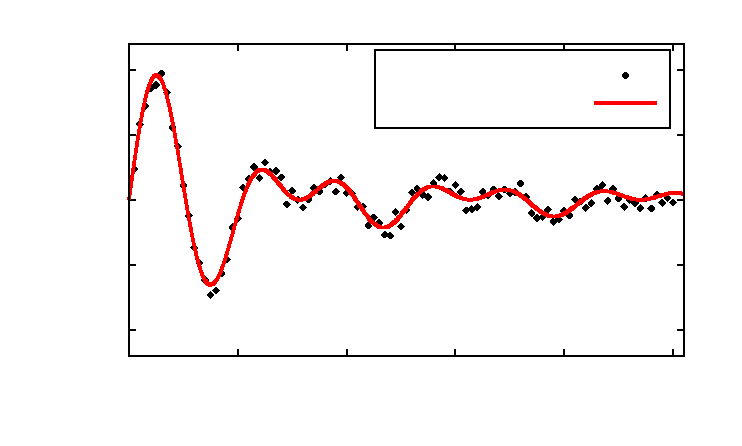
\includegraphics{nonlin-fit-example}}%
    \gplfronttext
  \end{picture}%
\endgroup

						\end{figure}
				\end{tcolorbox}				
			\end{frame}
		
		% subsection idee_des_ausgleichsproblems (end)

		\subsection{Das etwas allgemeinere Ausgleichsproblem} % (fold)
		\label{sub:das_etwas_allgemeinere_ausgleichsproblem}

			\begin{frame}
				\frametitle{Das etwas allgemeinere Ausgleichsproblem}

				\begin{tcolorbox}[title = Ausgleichsproblem mit Methode der kleinsten Quadrate]
					Für $n,m\in\SN, m\leq n$, eine gegebene Parametermenge $U\subset\SR^m$ und eine gegebene Residuen-Funktion $r:U\longrightarrow\SR^n$ ist das Ausgleichsproblem definiert durch
					\[ \min \set{\norm{r(\lambda)}^2_2}{\lambda\in U} \]
				\end{tcolorbox}
			\end{frame}
		
		% subsection das_etwas_allgemeinere_ausgleichsproblem (end)

	% section mathematische_grundlagen (end)

	\section{Lösungsverfahren}

	\subsection{Gauss-Newton-Verfahren} % (fold)
	\label{sec:gauss_newton_verfahren}
	
		\begin{frame}
			\frametitle{Gauß-Newton-Verfahren}

			\begin{tcolorbox}[title=Bedingungen für Minimum]
				\[ \nabla s(\lambda^\star) = 0 \]
				\[ \Deriv\curvb{\nabla s}(\lambda^\star) \text{ ist positiv definit} \]
			\end{tcolorbox}
		\end{frame}

		\begin{frame}
			
			\begin{tcolorbox}[colframe=black,colbacktitle=white,coltitle=black, attach boxed title to top center={yshift=-2mm},enhanced, titlerule=0.1pt, boxrule=0.5pt, breakable, arc=5pt,title=Algorithmus:\quad Gauß-Newton-Verfahren]
				Eingabe: $r:\SR^m\longrightarrow\SR^n,\quad \lambda^{(0)}\in\SR^m$

				\begin{enumerate}[label=\normalfont (\arabic*)]
					\item Setze $k=0$.
					\item Berechne $r\curvb{\lambda^{(k)}}, \Deriv r\curvb{\lambda^{(k)}}$.
					\label{schritt}
					\item Bestimme den Korrekturvektor $\xi^{(k)}$ gemäß
						\[ \boxb{ \transp{\curvb{\Deriv r}}\Deriv r }\curvb{\lambda^{(k)}} \xi^{(k)} = -\boxb{ \transp{\curvb{\Deriv r}}r }\curvb{\lambda^{(k)}} \]
					\item Setze $\lambda^{(k+1)} = \lambda^{(k)} + \xi^{(k)}$.
					\item Setze $k=k+1$.
					\item Gehe zu Schritt \ref{schritt}, wenn
						\[ k < k_\m{max} \quad \wedge \quad \norm{\xi^{(k)}}_2^2 > \delta_\m{min} \]
				\end{enumerate}
			\end{tcolorbox}

		\end{frame}

	% section gauss_newton_verfahren (end)

	\subsection{Levenberg-Marquardt-Verfahren} % (fold)
	\label{sec:levenberg_marquardt_verfahren}
	
		\begin{frame}
			\frametitle{Levenberg-Marquardt-Verfahren}

			\begin{tcolorbox}[title = korrigierte Normalengleichung]
				\[ \boxb{ \transp{\curvb{\Deriv r}}\Deriv r + \mu^2\idmat }\curvb{\lambda^{(k)}} \xi^{(k)} = -\boxb{ \transp{\curvb{\Deriv r}}r }\curvb{\lambda^{(k)}} \]
			\end{tcolorbox}

			\begin{itemize}[label=$\circ$]
				\item $\mu$ soll hier adaptiv gewählt werden
				\item obere und untere Schranken $\beta_0,\beta_1$ werden benötigt
			\end{itemize}
		\end{frame}

		\begin{frame}
			\frametitle{Levenberg-Marquardt-Verfahren}

			\begin{tcolorbox}[title = relative Residualänderung]
				\[ \varepsilon_\mu = \frac{ \norm{r\curvb{\lambda^{(k)}}}^2_2 - \norm{r\curvb{\lambda^{(k)}+\xi^{(k)}}}^2_2 }{ \norm{r\curvb{\lambda^{(k)}}}^2_2 - \norm{r\curvb{\lambda^{(k)}} + \Deriv r\curvb{\lambda^{(k)}}\xi^{(k)}}^2_2 } \]
			\end{tcolorbox}
		\end{frame}

		\begin{frame}
			\begin{tcolorbox}[colframe=black,colbacktitle=white,coltitle=black, attach boxed title to top center={yshift=-2mm},enhanced, titlerule=0.1pt, boxrule=0.5pt, breakable, arc=5pt,title=Algorithmus:\quad Levenberg-Marquardt-Verfahren Teil 1]
				Eingabe: $r:\SR^m\longrightarrow\SR^n,\quad \lambda^{(0)}\in\SR^m$

				\begin{enumerate}[label=\normalfont (\arabic*)]
					\item Setze $k=0$.
					\item Berechne $r\curvb{\lambda^{(k)}}, \Deriv r\curvb{\lambda^{(k)}}$.
					\label{lm-schritt}
					\item 
					\label{lm-corr}
					Bestimme den Korrekturvektor $\xi^{(k)}$ gemäß
						\[ \boxb{ \transp{\curvb{\Deriv r}}\Deriv r + \mu^2\idmat }\curvb{\lambda^{(k)}} \xi^{(k)} = -\boxb{ \transp{\curvb{\Deriv r}}r }\curvb{\lambda^{(k)}} \]
				\end{enumerate}
			\end{tcolorbox}

		\end{frame}

		\begin{frame}
			
			\begin{tcolorbox}[colframe=black,colbacktitle=white,coltitle=black, attach boxed title to top center={yshift=-2mm},enhanced, titlerule=0.1pt, boxrule=0.5pt, breakable, arc=5pt,title=Algorithmus:\quad Levenberg-Marquardt-Verfahren Teil 2]

				\begin{enumerate}[label=\normalfont (\arabic*), resume]
					\item Berechne $\varepsilon_\mu$ und teste, ob die Korrektur akzeptabel ist.
						\[ \varepsilon_\mu = \frac{ \norm{r\curvb{\lambda^{(k)}}}^2_2 - \norm{r\curvb{\lambda^{(k)}+\xi^{(k)}}}^2_2 }{ \norm{r\curvb{\lambda^{(k)}}}^2_2 - \norm{r\curvb{\lambda^{(k)}} + \Deriv r\curvb{\lambda^{(k)}}\xi^{(k)}}^2_2 } \]
						\begin{enumerate}[label=\normalfont (\roman*)]
							\item Fall $\varepsilon_\mu \leq \beta_0$: Setze $\mu = 2\mu$ und gehe zu \ref{lm-corr}.
							\item Fall $\varepsilon_\mu \geq \beta_1$: Setze $\mu = \frac{\mu}{2}$.
						\end{enumerate}
					\item Setze $\lambda^{(k+1)} = \lambda^{(k)} + \xi^{(k)}$.
					\item Setze $k=k+1$.
					\item Gehe zu Schritt \ref{lm-schritt}, wenn
						\[ k < k_\m{max} \quad \wedge \quad \norm{\xi^{(k)}}_2^2 > \delta_\m{min} \]
				\end{enumerate}
			\end{tcolorbox}

		\end{frame}

	% section levenberg_marquardt_verfahren (end)

	\subsection{Simulated Annealing} % (fold)
	\label{sub:simulated_annealing}
	
		\begin{frame}
			\frametitle{Simulated Annealing}

			\begin{itemize}[label=$\circ$]
				\item 
			\end{itemize}
		\end{frame}

		\begin{frame}
			\begin{tcolorbox}[colframe=black,colbacktitle=white,coltitle=black, attach boxed title to top center={yshift=-2mm},enhanced, titlerule=0.1pt, boxrule=0.5pt, breakable, arc=5pt,title=Algorithmus:\quad Simulated Annealing]
				Eingabe: $r:\SR^m\longrightarrow\SR^n,\quad \lambda_0\in\SR^m$

				\begin{enumerate}[label=\normalfont (\arabic*)]
					\item Berechne $c_0 = \norm{ r\curvb{ \lambda_0 } }_2^2$.
					\item Setze $T = T_0$ und $i=0$.
					\item \label{sa-for} Bestimme einen zufälligen Parameter $\lambda_1$.
					\item Berechne $c_1 = \norm{ r\curvb{ \lambda_1 } }_2^2$.
					\item
						\begin{itemize}
							\item Fall $c_1 < c_2$: Setze $\lambda_0 = \lambda_1$.
							\item Fall $c_1 \geq c_2$: Berechne
								\[ p = \exp\curvb{ \frac{c_0 - c_1}{T} } \]
								und setze $\lambda_0 = \lambda_1$ mit Wahrscheinlichkeit $p$. 
						\end{itemize}
					\item Setze $i=i+1$ und gehe zu Schritt \ref{sa-for}, wenn $i < i_\m{max}$.
					\item Setze $T=\alpha T$ und gehe zu Schritt \ref{sa-for}, wenn $T > T_\m{min}$.
				\end{enumerate}
			\end{tcolorbox}
		\end{frame}

	% subsection simulated_annealing (end)

	\section{Fazit und Zusammenfassung} % (fold)
	\label{sec:fazit_und_zusammenfassung}
	
		\begin{frame}
			\frametitle{Fazit und Zusammenfassung}
			

			\begin{itemize}[label=$\circ$]
				\item es gibt selte eine geschlossene Form der Problemstellung
				\[ \implies \quad \text{iterative Verfahren werden benötigt} \]
				\item nichtlineare Ausgleichsprobleme erfordern je nach gewählter Parameterfunktion spezifische Verfahren
				\[ \implies \quad \text{adaptive Steuerung gewählter Parameter nötig} \]
				\item viele Verfahren finden nur lokale Minima
				\item Startwertproblem
			\end{itemize}
		\end{frame}

	% section fazit_und_zusammenfassung (end)

	\section{Referenzen} % (fold)
	\label{sec:referenzen}
		
		\begin{frame}
			\frametitle{Referenzen}

			\begin{itemize}[label=$\circ$]
				\item Hermann, \textit{Numerische Mathematik}, 3.Auflage
				\item \url{http://en.wikipedia.org/wiki/Gauss-Newton_algorithm}
				\item \url{http://en.wikipedia.org/wiki/Levenberg-Marquardt_algorithm}
				\item \url{http://en.wikipedia.org/wiki/Simulated_annealing}
				\item Funken, \textit{Numerik III}, Skript Universität Ulm, 2012/2013
				\item \url{katrinaeg.com/simulated-annealing.html}
				\item Kincaid und Cheney, \textit{Numerical Analysis}, 3.Edition
			\end{itemize}
		\end{frame}

	% section referenzen (end)

\end{document}